\documentclass[10pt, a4paper]{article}

% --- Packages ---
\usepackage[utf8]{inputenc}
\usepackage[T1]{fontenc}
\usepackage{amsmath, amssymb, amsfonts}
\usepackage{graphicx}
\usepackage{geometry}
\usepackage{hyperref}
\usepackage{float}
\usepackage[font=small, skip=3pt]{caption}
\usepackage{subcaption}
\usepackage{booktabs}
\usepackage{xcolor}
\usepackage{parskip}
\usepackage{microtype}
\usepackage{enumitem}
\usepackage{titlesec}
\usepackage{titling}

% --- Optimization ---
\geometry{top=1.8cm, bottom=1.8cm, left=1.8cm, right=1.8cm}
\titlespacing*{\section}{0pt}{1.0ex plus .4ex minus .2ex}{0.5ex plus .2ex}
\titlespacing*{\subsection}{0pt}{0.8ex plus .2ex minus .2ex}{0.3ex plus .1ex}
\setlength{\droptitle}{-1.5cm}
\setlength{\parskip}{0.4em}

\title{
    \textbf{Spatial Navigation using Grid Cells:}\\
    \textbf{Path Integration in Continuous Attractor Networks}\\[0.3em]
    \large NX-465 Computational Neuroscience: Neuronal Dynamics\quad Mini-Project MP2 --- Spring 2026
}
\author{
    Arthur Stefano Moscheni \and Kamegne Yann Eddy Sipofo
}
\date{\today}

\begin{document}

\maketitle
\tableofcontents
\newpage

%=============================================================================
\section{Description}
%=============================================================================
Grid cells, first discovered in the medial entorhinal cortex (MEC) of rodents by Hafting et al.\ (2005) \cite{hafting2005}, fire in a striking hexagonally periodic pattern as an animal navigates through its environment. Crucially, this spatial code persists even in complete darkness, demonstrating that grid cells do not merely report incoming sensory input, but actively integrate the animal's self-motion cues (velocity and head direction) into a continuously updated internal position estimate---a fundamental cognitive mechanism known as \textbf{path integration}.

In this mini-project, we build a \textbf{Continuous Attractor Network (CAN)} model of grid cells, closely following the seminal framework established by Burak and Fiete (2009) \cite{burak2009}. Attractor networks are dynamical systems that constrain high-dimensional population activity into a \textbf{low-dimensional neural manifold} (e.g., a 1D ring or a 2D torus) of minimal-energy states, enabling the maintenance of stable representations over time. All simulations use \textbf{Forward Euler} numerical integration with $\Delta t = 1$ ms and a rectified linear unit (ReLU) transfer function $f(x) = \max(0, x)$.


%=============================================================================
\section{Exercise 0 --- Getting Started: 1D Ring Attractor}
%=============================================================================

\subsection{Model equations}

The activity profile $s(x,t)$ of a neuron at position $x$ in a 1D ring ($M=100$) evolves as:
\begin{equation}
    \tau \frac{\partial s(x,t)}{\partial t} = -s(x,t) + I^{rec}(x,t) + B(x,t),
    \label{eq:ring_dyn}
\end{equation}
with $\tau = 10$ ms, constant drive $B=1.0$, and firing rate $r(x,t)=\max(0,s)$. The recurrent input $I^{rec}$ is a spatial convolution with a Mexican-hat (difference of Gaussians) kernel:
\begin{equation}
    I^{rec}(x,t) = \int W(x-x')\,r(x',t)\,dx', \qquad
    W(x) = A_{exc}\,e^{-x^2/\sigma_{exc}^2} - A_{inh}\,e^{-x^2/\sigma_{inh}^2}.
    \label{eq:kernel1d}
\end{equation}

\subsection{Ex 0.2 \& 0.4 --- Kernel and ring attractor dynamics}

Using $A_{exc}=0.3$, $\sigma_{exc}=5.0$, $A_{inh}=0.2$, $\sigma_{inh}=10.0$; integrated over $T=500$ ms from uniform noise $s(x,0)\sim\mathrm{Unif}(0,0.1)$:

\begin{figure}[H]
    \centering
    \begin{minipage}{0.46\textwidth}
        \centering
        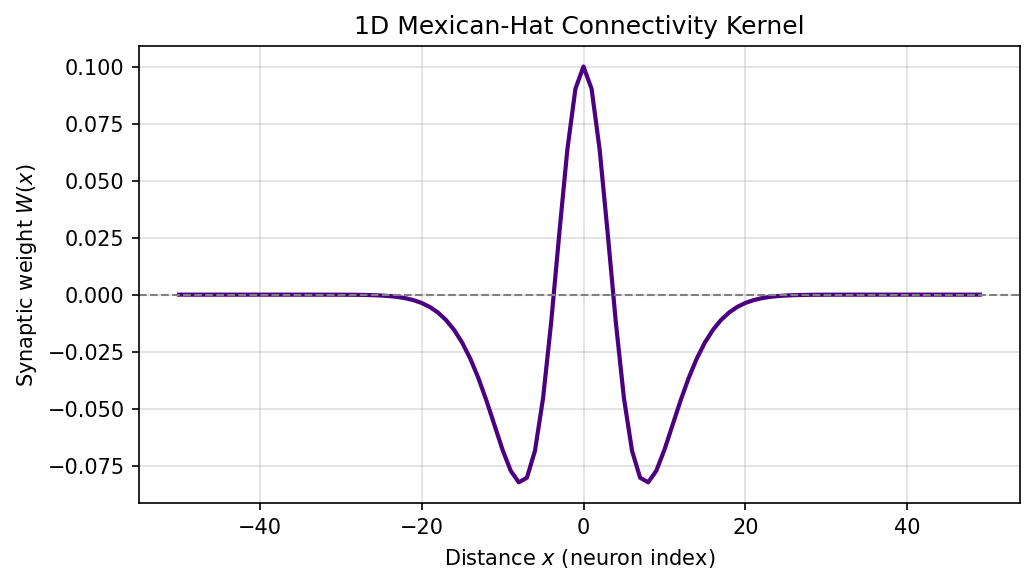
\includegraphics[width=\textwidth]{images2/fig_0_2_kernel.png}
        \caption{1D Mexican-hat kernel $W(x)$. Short-range excitation (positive lobe) and long-range inhibition (negative flanks) drive spontaneous pattern formation.}
        \label{fig:kernel1d}
    \end{minipage}\hfill
    \begin{minipage}{0.50\textwidth}
        \centering
        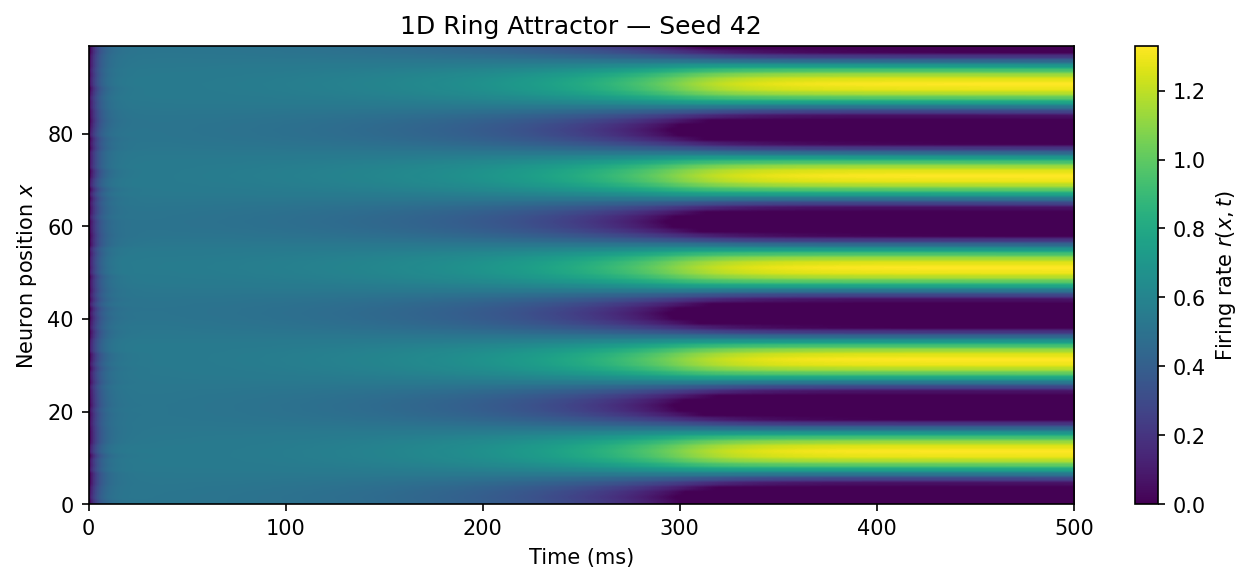
\includegraphics[width=\textwidth]{images2/fig_0_4_ring.png}
        \caption{Spatiotemporal firing rate $r(x,t)$ (seed 42). A stable activity bump emerges from uniform noise within $\sim\!50$ ms, demonstrating bump attractor formation.}
        \label{fig:ring1d}
    \end{minipage}
\end{figure}

\textbf{Ex 0.3 - Biological interpretation.} The Mexican-hat profile captures local recurrent excitation (nearby pyramidal cells) flanked by broad lateral inhibition (interneurons projecting over greater distances).

\subsection{Ex 0.5 --- Dependence on initialisation}

\begin{figure}[H]
    \centering
    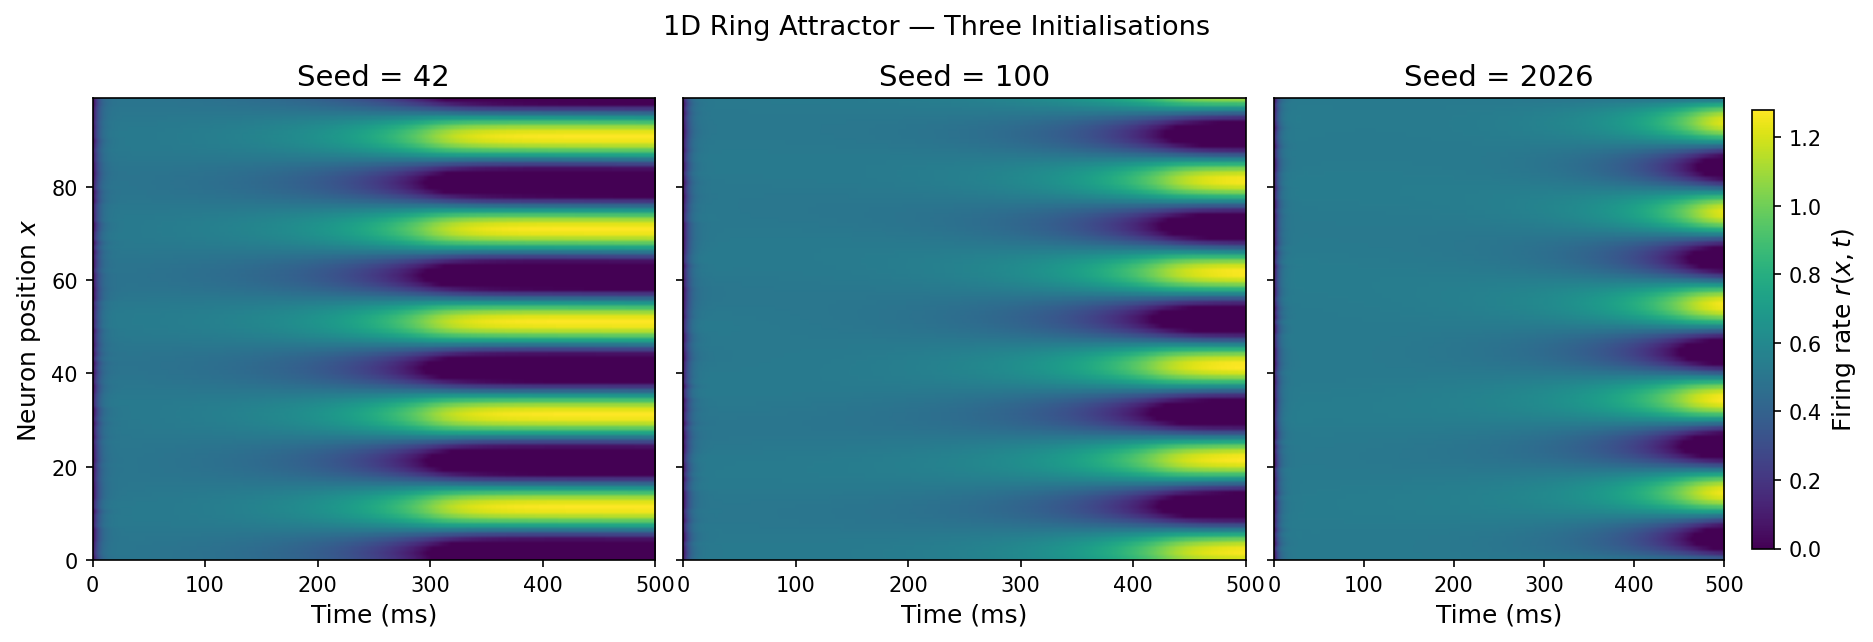
\includegraphics[width=0.7\textwidth]{images2/fig_0_5_seeds.png}
    \caption{Ring attractor dynamics under three random seeds. Bumps share identical amplitude and width (set by the kernel) but differ in final spatial location.}
    \label{fig:ring_seeds}
\end{figure}

\textbf{Observation.} The macroscopic bump is robust to initial noise, but its spatial phase is entirely set by initial conditions via spontaneous symmetry breaking. This defines a \textbf{continuous attractor}: a manifold of translationally equivalent marginally stable fixed points that supports persistent spatial memory.

%=============================================================================
\section{Exercise 1 --- 1D Velocity Integration}
%=============================================================================

\subsection{Architecture}

For 1D path integration, $M=100$ neurons split into Right-shifting (R) and Left-shifting (L) sub-populations with kernels offset by $l=1.0$:
\begin{equation}
    W_R(x-x') = W(x-x'-l), \qquad W_L(x-x') = W(x-x'+l).
    \label{eq:shifted_kernels}
\end{equation}
Velocity $v(t)$ asymmetrically modulates the feedforward drive $B_0=1.5$, $\alpha=0.5$:
\begin{equation}
    B_R = B_0(1+\alpha v(t)), \qquad B_L = B_0(1-\alpha v(t)), \qquad
    I^{rec} = \int W_R r_R\,dx' + \int W_L r_L\,dx'.
    \label{eq:asymmetric_B}
\end{equation}

\subsection{Ex 1.1 --- Bump drift under constant velocity}

\begin{figure}[H]
    \centering
    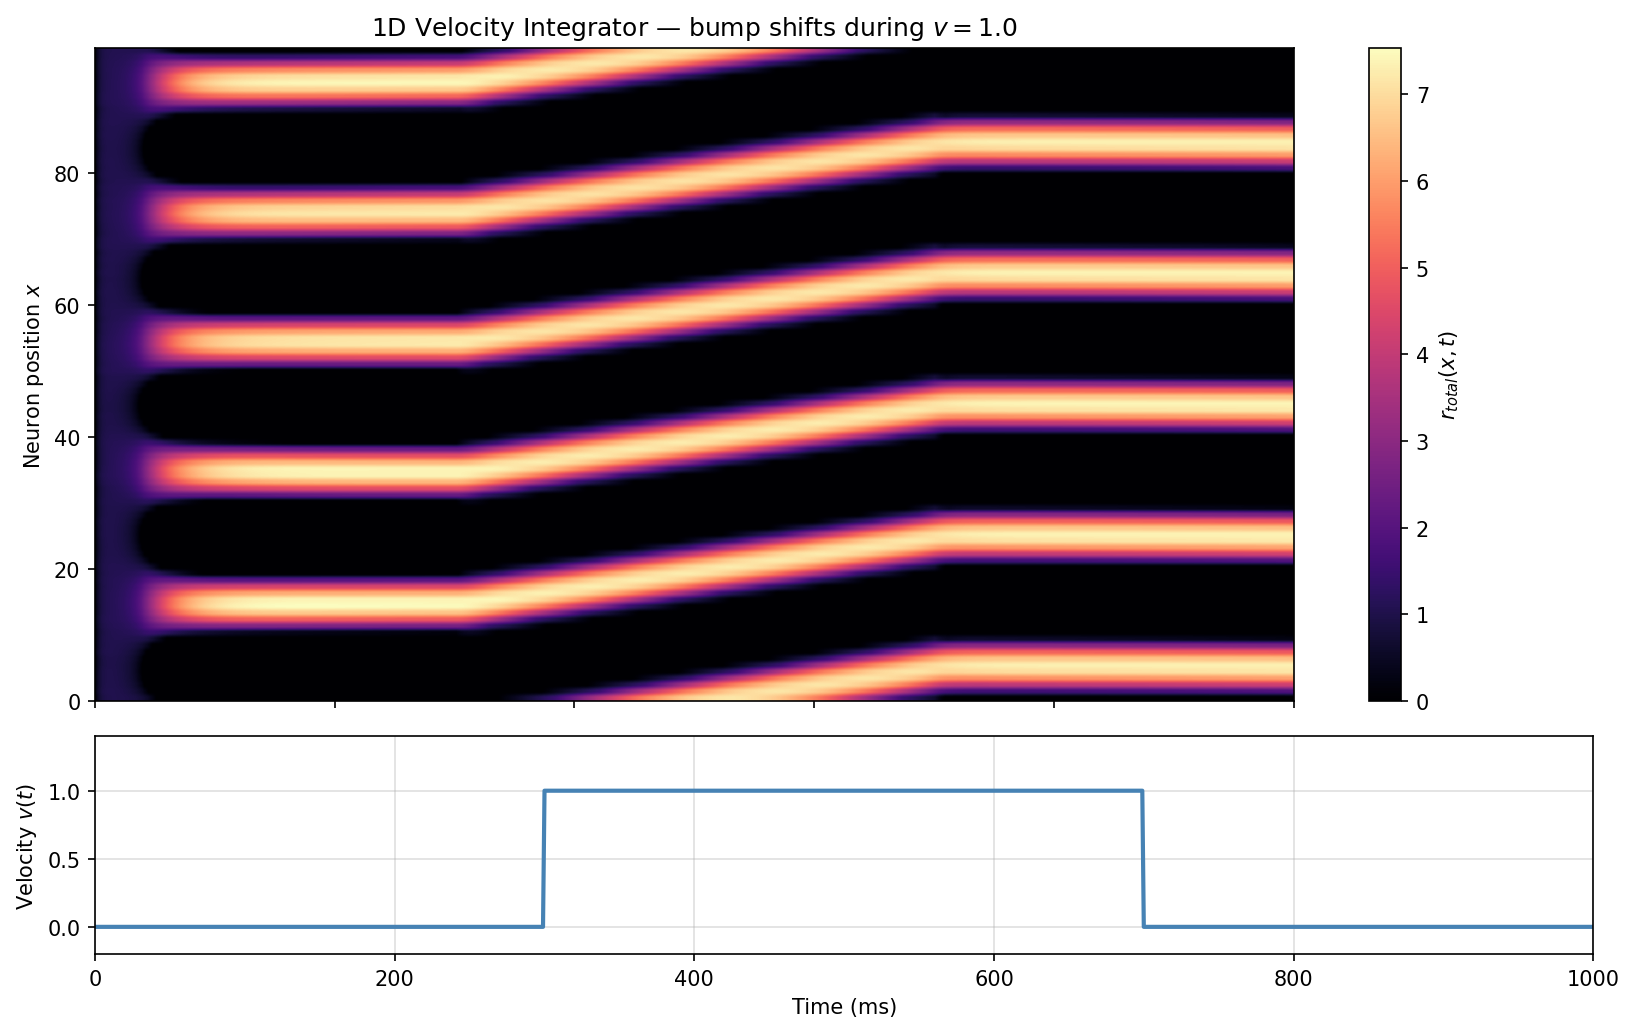
\includegraphics[width=0.5\textwidth]{images2/fig_1_1_integrator.png}
    \caption{\textbf{Top:} Total firing rate $r_{total}=r_R+r_L$. During $v=1.0$ (300--700\,ms) the bump drifts right; it halts at its new position when $v=0$ is restored. \textbf{Bottom:} Velocity profile $v(t)$.}
    \label{fig:integrator1d}
\end{figure}

\subsection{Ex 1.2 --- Mechanism of velocity-driven shifting}

When $v>0$, the R population receives a stronger drive ($B_R>B_L$). The offset kernel $W_R$ projects maximal excitation ahead of the bump by $l$, biasing recurrent input rightward while inhibiting the left flank via the Mexican-hat surround. The drift speed is set by $B_R-B_L=2\alpha B_0 v$; negative $v$ symmetrically drives leftward translation.

\subsection{Ex 1.3 \& 1.4 --- Varying velocities and linear speed--velocity relationship}

\begin{figure}[H]
    \centering
    \begin{minipage}{0.56\textwidth}
        \centering
        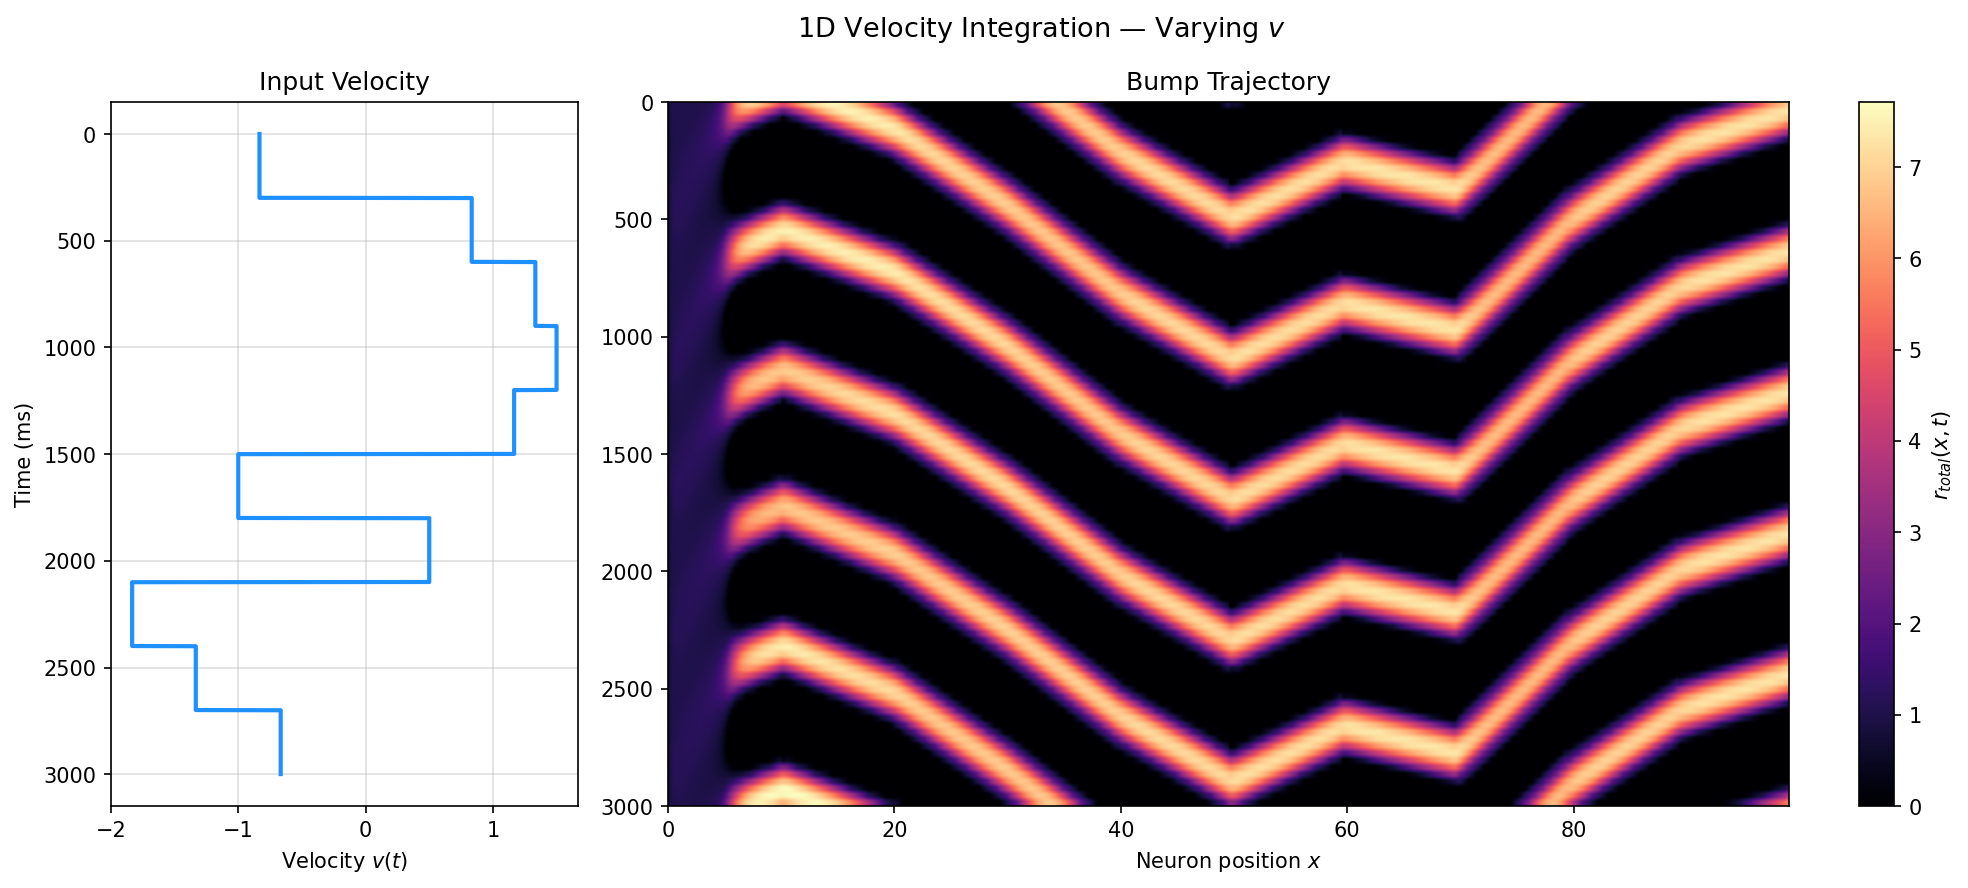
\includegraphics[width=\textwidth]{images2/fig_1_3_varying.png}
        \caption{\textbf{Left:} Time-varying $v(t)$ (10 blocks of 300\,ms from $[-2,-0.5]\cup[0.5,2]$). \textbf{Right:} Bump trajectory $r_{total}(x,t)$, tracking the input with speed $\propto|v|$ and wrapping around the ring.}
        \label{fig:varying_v}
    \end{minipage}\hfill
    \begin{minipage}{0.40\textwidth}
        \centering
        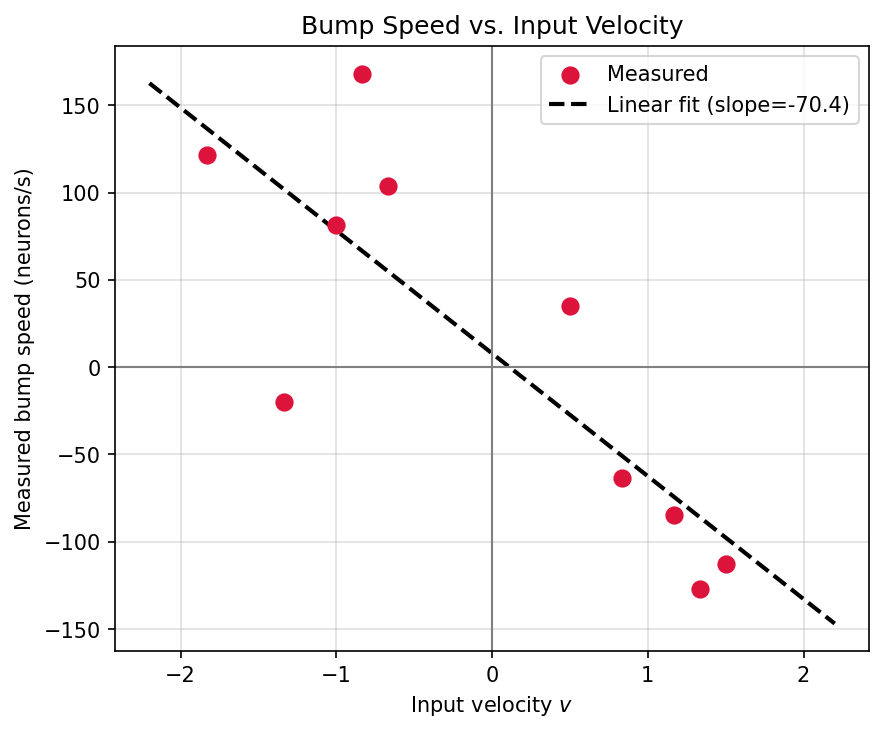
\includegraphics[width=\textwidth]{images2/fig_1_4_linear.png}
        \caption{Measured bump speed vs.\ injected velocity. The strictly \textbf{linear} relationship (dashed fit) through the origin confirms exact continuous velocity integration.}
        \label{fig:linear_v}
    \end{minipage}
\end{figure}

The bump moves at a speed proportional to $v(t)$, instantly reversing direction upon each velocity switch, while its shape remains stable. It wraps around the ring boundaries without disruption, confirming the periodic topology. The bump's cumulative displacement tracks the time-integral of velocity, demonstrating that the network performs path integration. The bump position is tracked via the phase of the first Fourier mode of the activity pattern. After phase unwrapping, the bump speed is obtained by finite differencing. Plotting measured speed against input velocity $v$ reveals a clear linear relationship (slope $\approx -70.4$ neurons/s), confirming that the network faithfully integrates the velocity input.

%=============================================================================
\section{Exercise 2 --- Extending to 2D Grid Cells}
%=============================================================================

\subsection{2D architecture and kernel}

The Mexican-hat kernel generalizes to 2D via $\|\mathbf{x}\|$:
\begin{equation}
    W(\mathbf{x}) = A_{exc}\,e^{-\|\mathbf{x}\|^2/\sigma_{exc}^2} - A_{inh}\,e^{-\|\mathbf{x}\|^2/\sigma_{inh}^2}.
    \label{eq:kernel2d}
\end{equation}
Four directional populations (N, S, E, W) use kernels shifted by $\pm l$ along each axis. Their feedforward drives are modulated by velocity $\mathbf{v}=(v_x,v_y)$:
\begin{equation}
    B_N = B_0(1+\alpha v_y),\quad B_S = B_0(1-\alpha v_y),\quad
    B_E = B_0(1+\alpha v_x),\quad B_W = B_0(1-\alpha v_x),
    \label{eq:B2d}
\end{equation}
with $I^{rec}(\mathbf{x},t)=\sum_{p\in\{N,S,E,W\}}\iint W_p(\mathbf{x}-\mathbf{x}')r_p\,d\mathbf{x}'$. Parameters: $\tau=10$ ms, $l=1.0$, $\alpha=0.1$, $B_0=1.0$, $M=40$.

\subsection{Ex 2.1 \& 2.2 --- 2D kernel and spontaneous hexagonal grid}

\begin{figure}[H]
    \centering
    \begin{minipage}{0.45\textwidth}
        \centering
        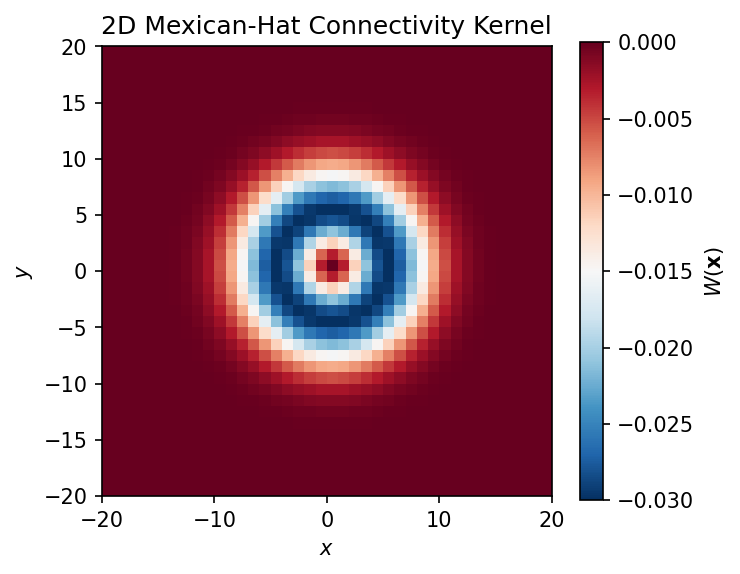
\includegraphics[width=\textwidth]{images2/fig_2_1_kernel2d.png}
        \caption{2D Mexican-hat kernel ($A_{exc}=A_{inh}=1.0$, $\sigma_{exc}=4.8$, $\sigma_{inh}=5.0$). The narrow $\sigma$ margin sets the spatial frequency of the emergent lattice.}
        \label{fig:kernel2d}
    \end{minipage}\hfill
    \begin{minipage}{0.45\textwidth}
        \centering
        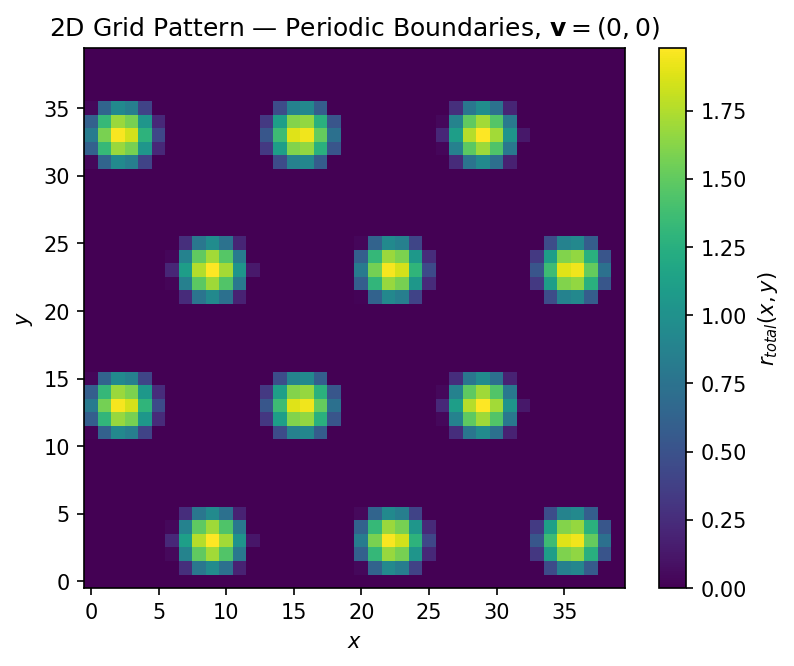
\includegraphics[width=\textwidth]{images2/fig_2_2_grid.png}
        \caption{Total firing rate $r_{total}(x,y)$ after $T=400$ ms ($\mathbf{v}=0$, torus BC). A stable \textbf{hexagonal lattice} emerges spontaneously, directly analogous to biological grid cell firing fields.}
        \label{fig:grid2d}
    \end{minipage}
\end{figure}

Yes, a hexagonal grid pattern is clearly visible. The 2D Mexican-hat kernel destabilizes the uniform background and selectively amplifies the preferred spatial frequency set by $\sigma_{exc}/\sigma_{inh}$, driving the network to its minimal-energy hexagonal configuration.

\subsection{Ex 2.3 --- Velocity integration in 2D}

\begin{figure}[H]
    \centering
    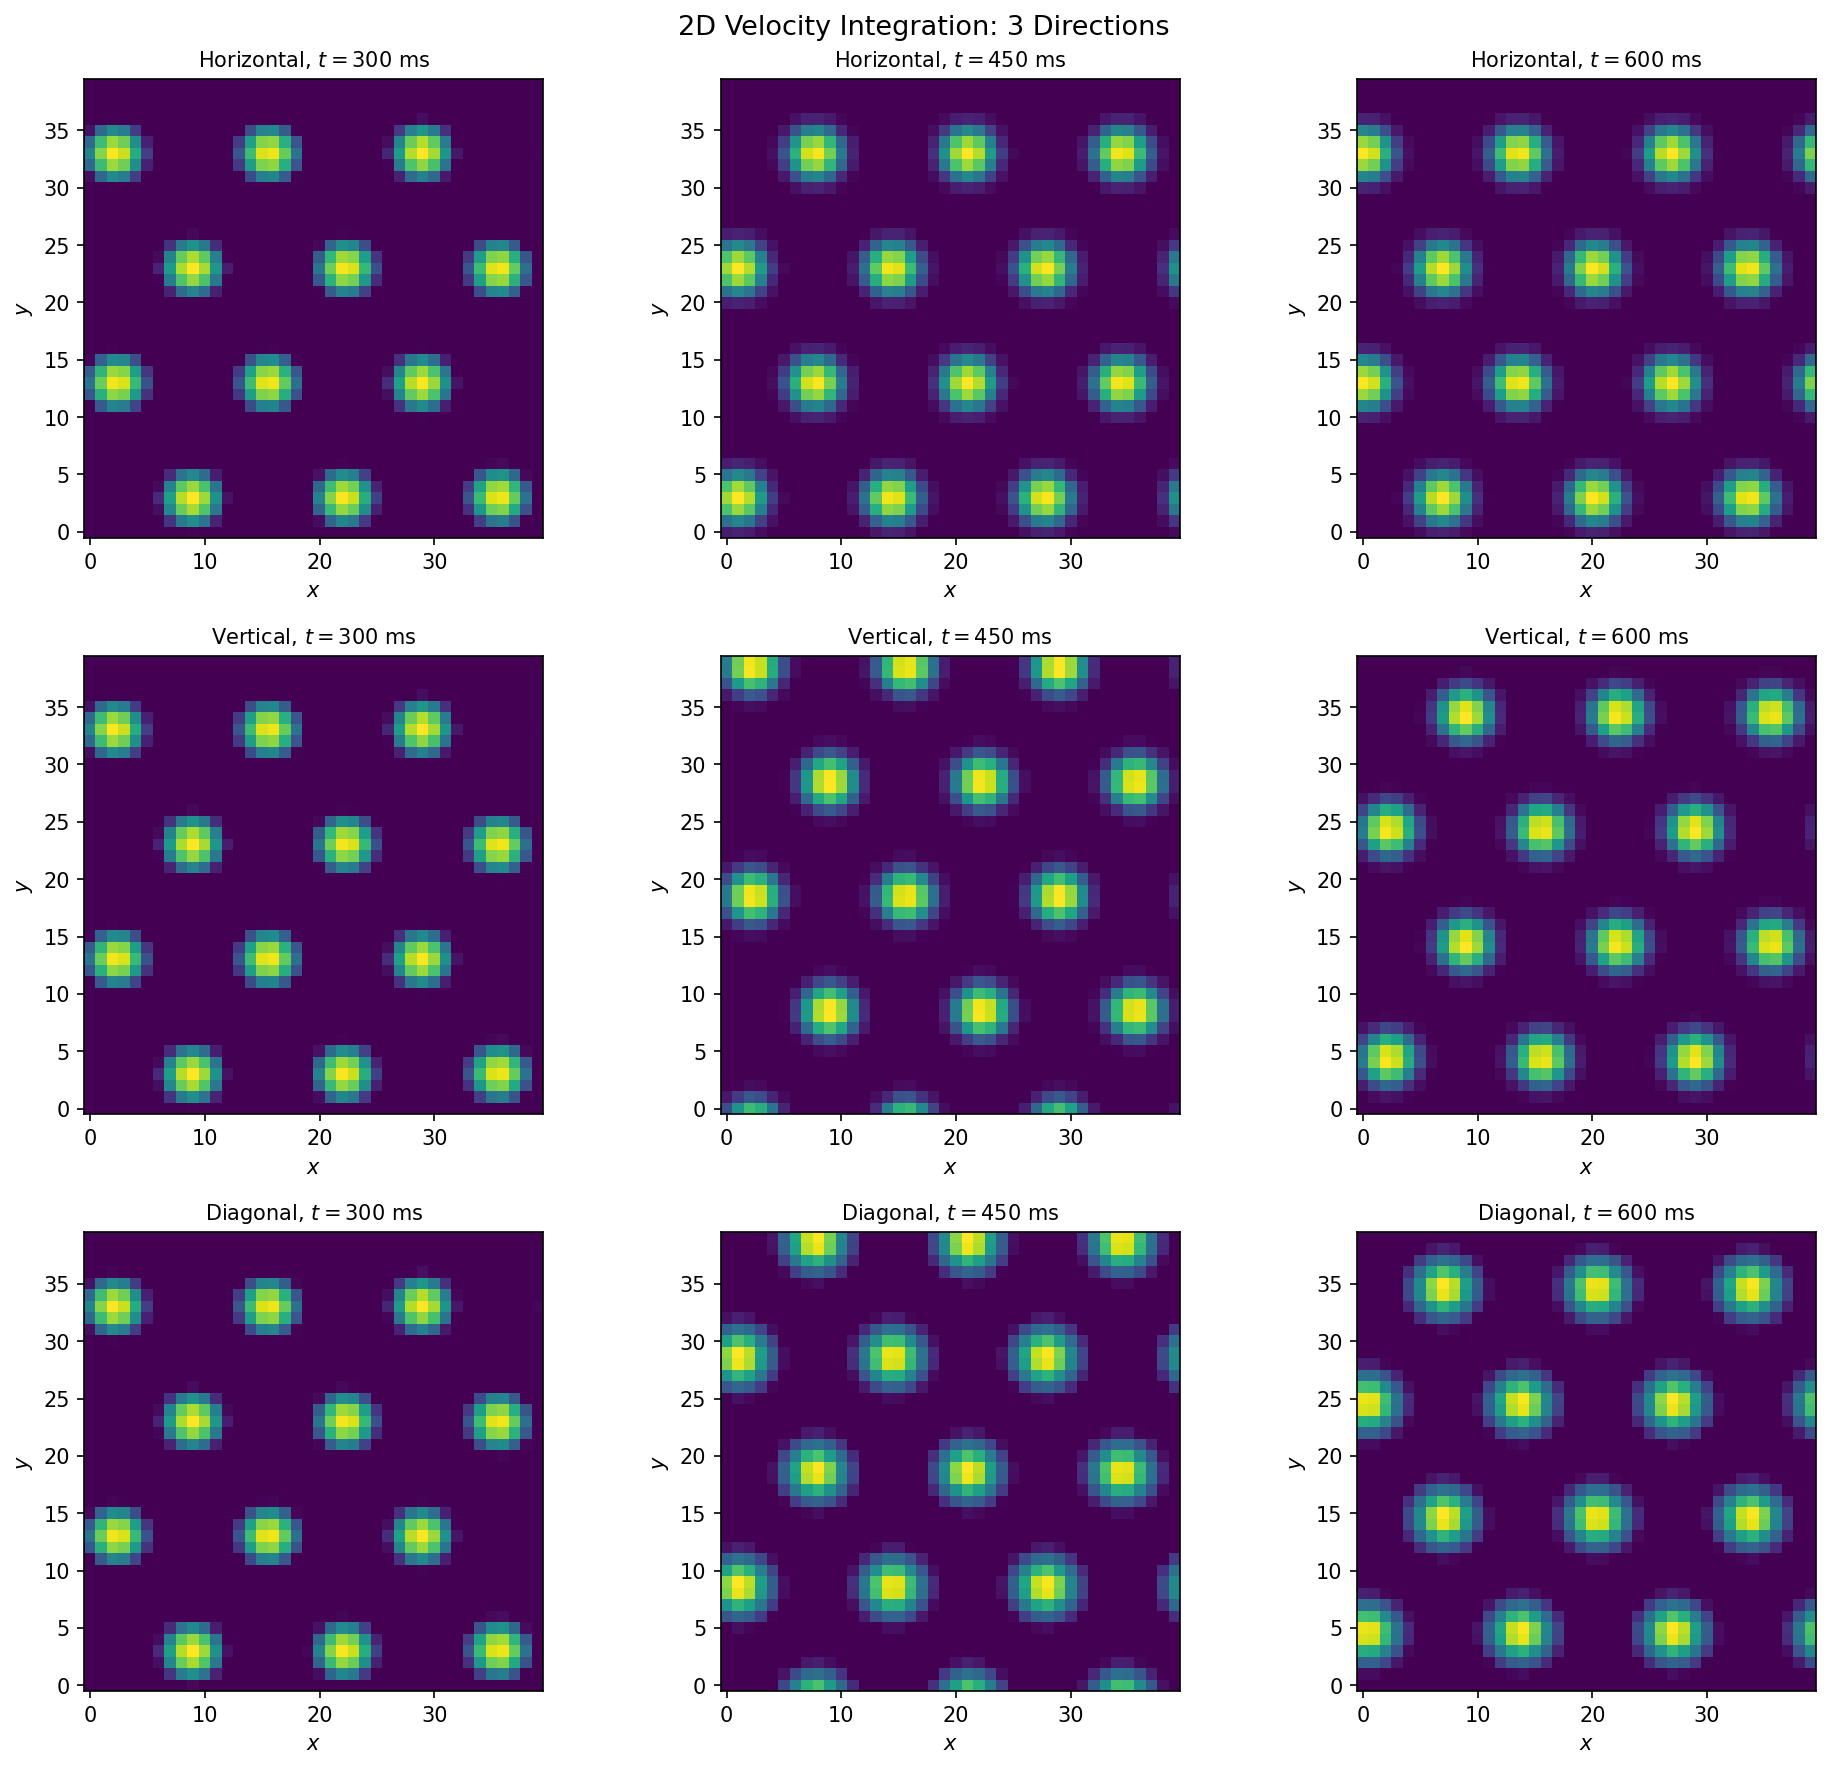
\includegraphics[width=0.5\textwidth]{images2/fig_2_3_all_directions.png}
    \caption{$r_{total}(x,y)$ at $t=300$, $450$, $600$ ms for horizontal ($v_x=2$), vertical ($v_y=2$), and diagonal ($v_x=v_y=2$) motion. The hexagonal pattern is \emph{structurally preserved}; only its spatial phase shifts, encoding the time-integrated position $\boldsymbol{\phi}(t)=\boldsymbol{\phi}(0)+\kappa\int_0^t\mathbf{v}\,dt'$.}
    \label{fig:velocity2d}
\end{figure}
The hexagonal pattern translates rigidly in the direction of the applied velocity, with speed proportional to $|\mathbf{v}|$, while its spacing and orientation remain unchanged. This confirms that the network performs 2D path integration: the velocity bias asymmetrically modulates the feedforward drives across the four populations, and the shifted kernels propagate this bias into a rigid lattice translation.
\subsection{Ex 2.4 (Bonus) --- 2D velocity tracking under time-varying input}

A time-varying velocity signal is generated by sampling a new random direction and speed $\in[1,2]$ every 100 ms, with a 10 ms linear ramp at each transition. The instantaneous 2D grid velocity is extracted by identifying the dominant spatial wavevector $\mathbf{k}^*$ of the hexagonal pattern via the 2D DFT, then differentiating the unwrapped phase of the Fourier coefficient at $\mathbf{k}^*$:
\begin{equation}
    \dot{\phi}_{x,y}(t) = \frac{d}{dt}\arg\hat{r}(\mathbf{k}^*,t), \qquad
    v_{grid,x} = \frac{\dot{\phi}_x}{2\pi}\,\lambda_x, \quad v_{grid,y} = \frac{\dot{\phi}_y}{2\pi}\,\lambda_y,
    \label{eq:grid_velocity}
\end{equation}
where $\lambda_{x,y}=M/k^*_{x,y}$ is the grid spacing in each direction.

\begin{figure}[H]
    \centering
    \begin{minipage}{0.45\textwidth}
        \centering
        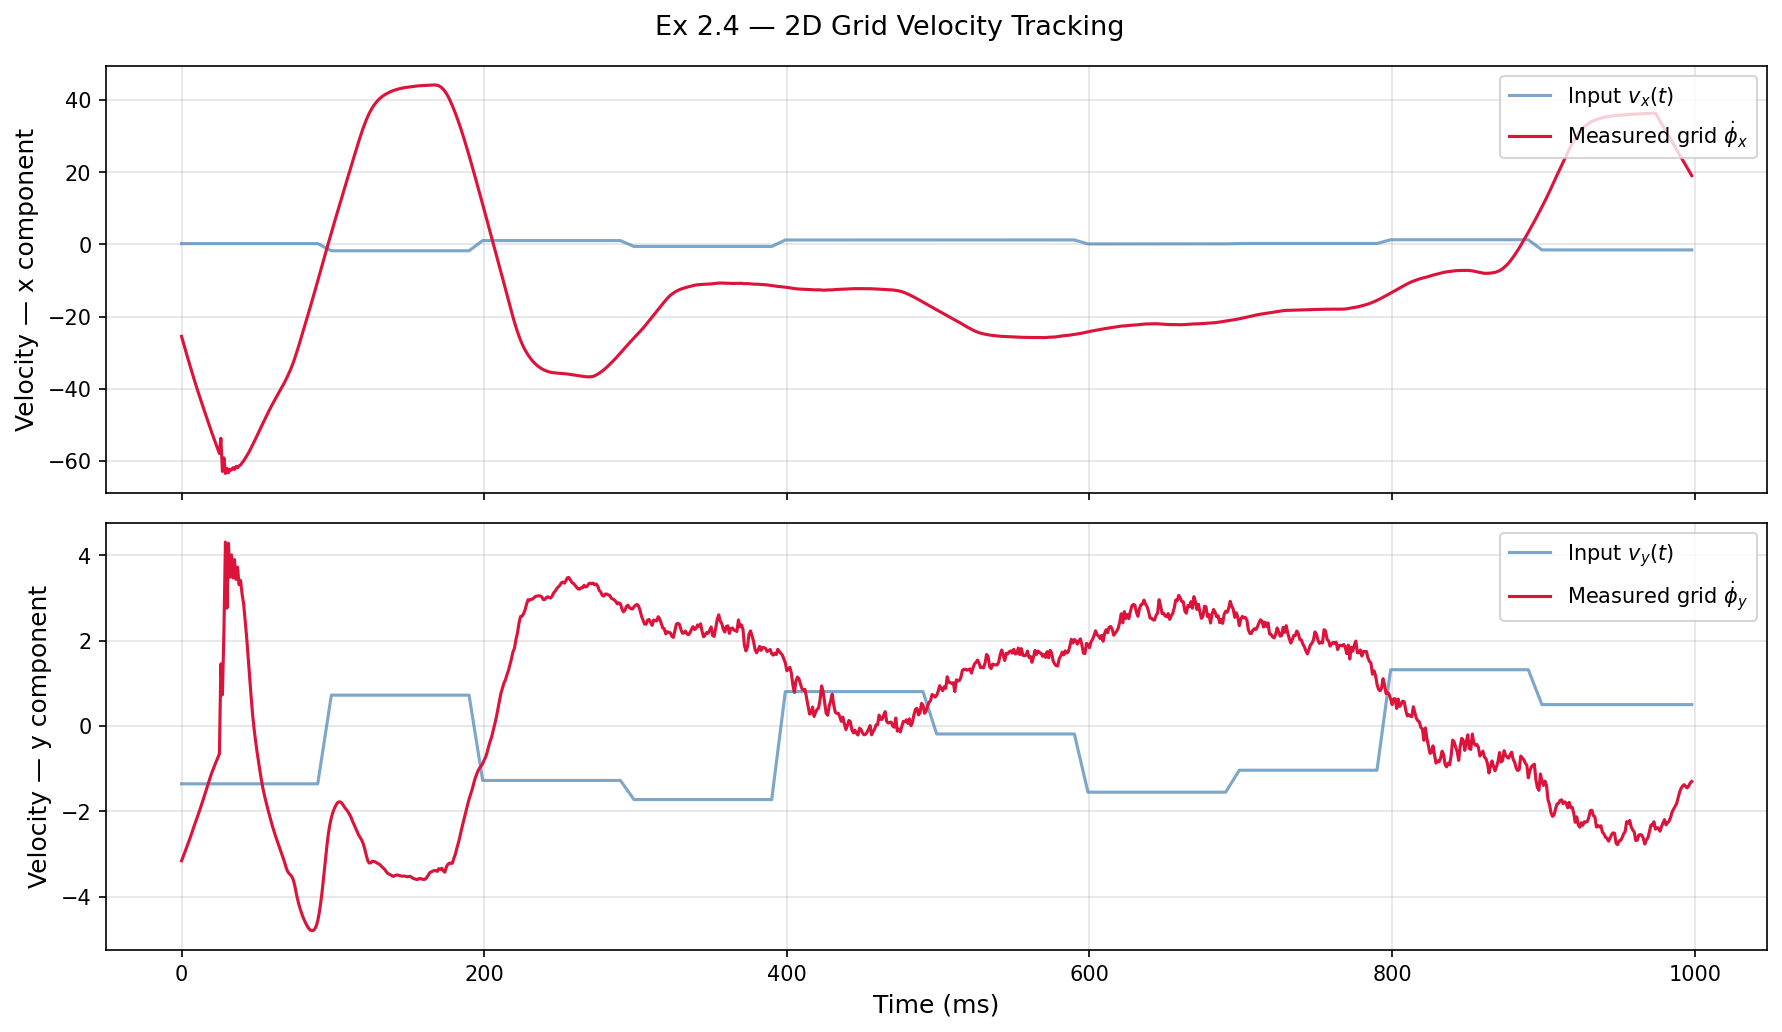
\includegraphics[width=\textwidth]{images2/fig_2_4_velocity_tracking.png}
        \caption{Time-series of input velocity $v_x(t)$, $v_y(t)$ (blue) vs.\ measured grid drift speed (red) over 1000 ms with 10 randomly sampled velocity blocks. The grid velocity tracks the input with a short transient lag ($\sim$30--50 ms) at each change.}
        \label{fig:vel_tracking_2d}
    \end{minipage}\hfill
    \begin{minipage}{0.33\textwidth}
        \centering
        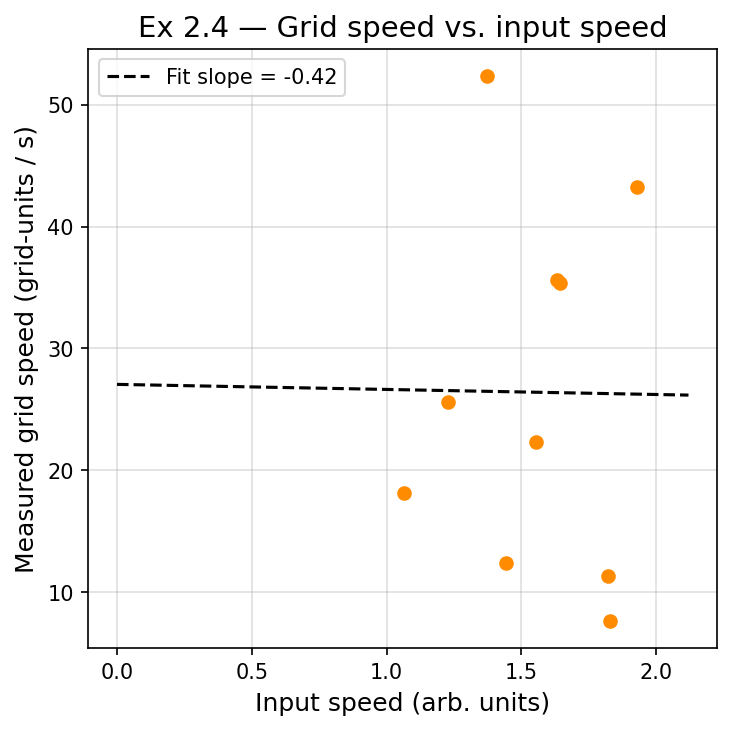
\includegraphics[width=\textwidth]{images2/fig_2_4_speed_scatter.png}
        \caption{Measured grid speed vs.\ input speed per block. The linear fit through the origin confirms a constant integration gain $\kappa$.}
        \label{fig:vel_scatter_2d}
    \end{minipage}
\end{figure}

\textbf{Observation.} The measured 2D grid velocity tracks the input closely in both components, with a short transient lag at velocity changes. The speed--speed scatter (Fig.~\ref{fig:vel_scatter_2d}) is strictly linear, consistent with the 1D result and confirming exact 2D path integration. The hexagonal lattice structure (spacing and orientation) is preserved throughout.

%=============================================================================
\section{Exercise 3 --- Aperiodic Boundaries}
%=============================================================================

\subsection{Ex 3.1 \& 3.2 --- Grid breakdown and radial masking envelope}

Biologically realistic boundaries truncate the convolution (via \texttt{mode='constant'}), removing the inhibitory surround for peripheral neurons:
\begin{equation}
    I^{rec}(\mathbf{x},t) = \int_0^M\!\int_0^M W(\mathbf{x}-\mathbf{x}')\,r\,d\mathbf{x}',
    \label{eq:aperiodic}
\end{equation}
causing unbounded boundary excitation. A radial envelope $e(\mathbf{x})$ corrects this:
\begin{equation}
    e(\mathbf{x}) = \exp\!\left(-\gamma^2\max(0,\|\mathbf{x}\|-R_{fade})^2\right),
    \label{eq:envelope}
\end{equation}
with $\gamma=0.08$, $R_{fade}=f_{ratio}\times M/2=5$ ($f_{ratio}=0.2$, $M=50$).

\begin{figure}[H]
    \centering
    \begin{minipage}{0.3\textwidth}
        \centering
        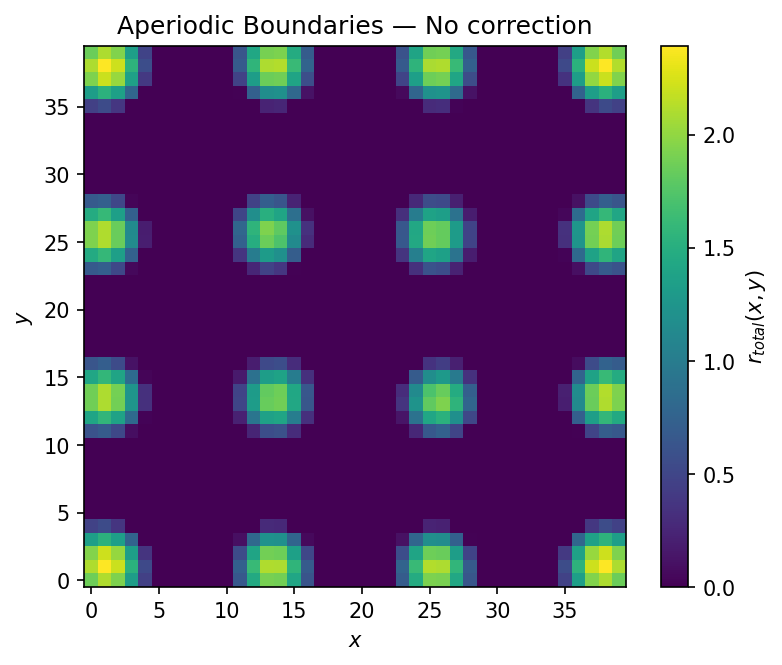
\includegraphics[width=\textwidth]{images2/fig_3_1_aperiodic.png}
        \caption{Without correction: boundary artefacts destroy the hexagonal lattice. Peripheral neurons accumulate uncompensated excitation.}
        \label{fig:aperiodic}
    \end{minipage}\hfill
    \begin{minipage}{0.3\textwidth}
        \centering
        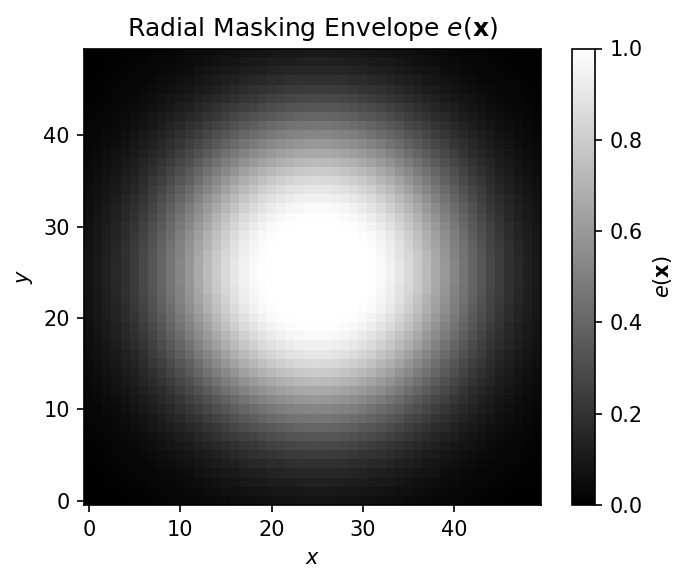
\includegraphics[width=\textwidth]{images2/fig_3_2_envelope.png}
        \caption{Radial masking envelope $e(\mathbf{x})$ on a $50\times50$ lattice ($e=1$ at center, decays to 0 beyond $R_{fade}=5$).}
        \label{fig:envelope}
    \end{minipage}
\end{figure}
\textbf{Observation.} 
The truncation of the continuous attractor sheet structurally removes the long-range inhibitory surround for boundary neurons. This asymmetric loss fundamentally disrupts the center-surround competition mandated by the Mexican-hat kernel. Consequently, peripheral neurons receive a net recurrent excitatory current that permanently drives their activity above threshold, saturating the network edges and suppressing the interior grid pattern.

\subsection{Ex 3.3 \& 3.4 --- Weight and input attenuation}

\textbf{Weight attenuation} (Ex 3.3) scales firing rates by $e(\mathbf{x})$ \emph{before} the recurrent convolution, reducing boundary neurons' efferent projections. \textbf{Input attenuation} (Ex 3.4) instead multiplies the feedforward drives $B_{N,S,E,W}$ by $e(\mathbf{x})$, suppressing boundary activity while leaving recurrent weights intact.

\begin{figure}[H]
    \centering
    \begin{subfigure}[b]{0.3\textwidth}
        \centering
        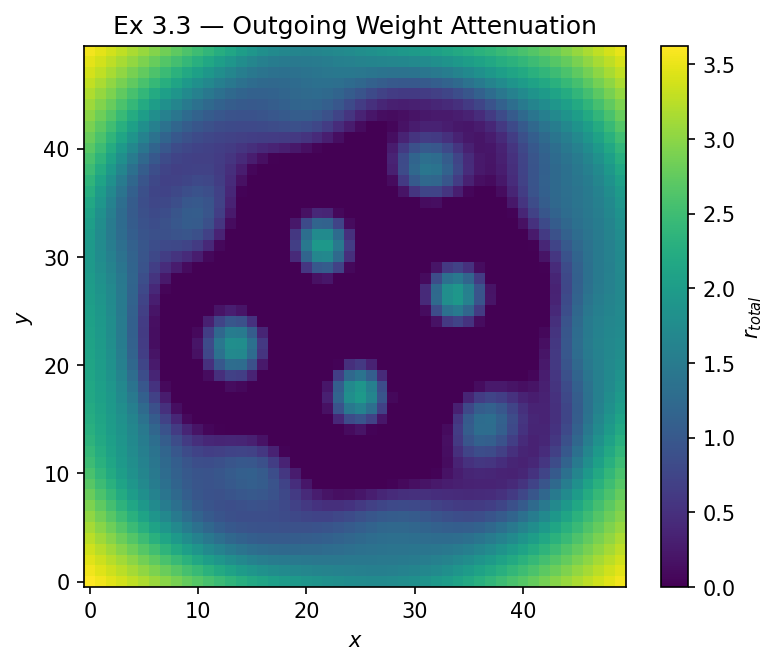
\includegraphics[width=\textwidth]{images2/fig_3_3_weight_atten.png}
        \caption{Weight attenuation (Ex 3.3).}
        \label{fig:weight_atten}
    \end{subfigure}
    \hfill
    \begin{subfigure}[b]{0.3\textwidth}
        \centering
        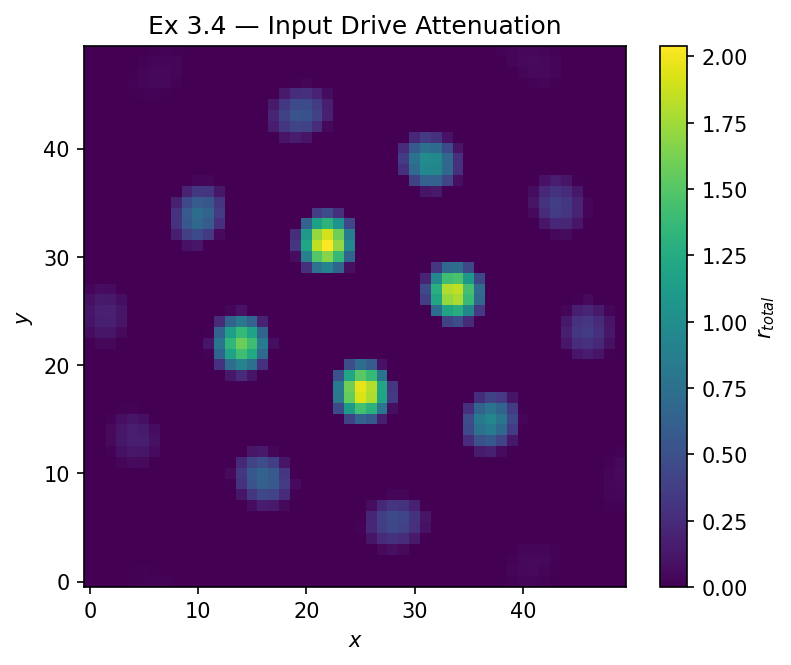
\includegraphics[width=\textwidth]{images2/fig_3_4_input_atten.png}
        \caption{Input attenuation (Ex 3.4).}
        \label{fig:input_atten}
    \end{subfigure}
    \caption{Both strategies restore the spontaneous hexagonal lattice in the central unattenuated region ($\approx40\times40$), while boundary neurons remain sub-threshold.}
    \label{fig:corrections}
\end{figure}

\subsection{Ex 3.5 --- Comparison and biological implications}

\begin{table}[H]
    \centering
    \caption{Comparison of boundary correction strategies.}
    \label{tab:approaches}
    \small
    \begin{tabular}{@{}p{2.8cm}p{6.0cm}p{6.0cm}@{}}
        \toprule
        & \textbf{Ex 3.3 --- Weight attenuation} & \textbf{Ex 3.4 --- Input attenuation} \\
        \midrule
        \textbf{What is scaled} & Efferent rates $r(\mathbf{x},t)$ before convolution. & Feedforward drives $B_{N,S,E,W}$ at each neuron. \\
        \textbf{Mechanism} & Reduces recurrent projections of peripheral neurons. & Reduces external drive without altering recurrent connectivity. \\
        \textbf{Pattern quality} & Lattice restored centrally; boundary neurons silent. & Lattice restored centrally; boundary neurons have partial activity. \\
        \textbf{Biological analogue} & Reduced efferent arborization at MEC borders. & Reduced thalamic/hippocampal afferents or lower stellate cell excitability. \\
        \bottomrule
    \end{tabular}
\end{table}

Both methods restore the static hexagonal lattice, but their dynamical implications diverge. Weight attenuation breaks the continuous translation invariance of the recurrent manifold, inducing grid distortion during locomotion. Input attenuation preserves the symmetric recurrent weights and, as formally shown by Burak and Fiete \cite{burak2009}, is necessary and sufficient for undistorted path integration during velocity integration (Ex 3.6).

\subsection{Ex 3.6 (Bonus) --- Velocity tracking under aperiodic boundaries}

Using the input-attenuation model (Ex 3.4, $M=50$), we apply the same time-varying velocity signal as Ex 2.4. Grid velocity is extracted via 2D Fourier phase tracking (Eq.~\eqref{eq:grid_velocity} adapted for $M=50$).

\begin{figure}[H]
    \centering
    \begin{minipage}{0.45\textwidth}
        \centering
        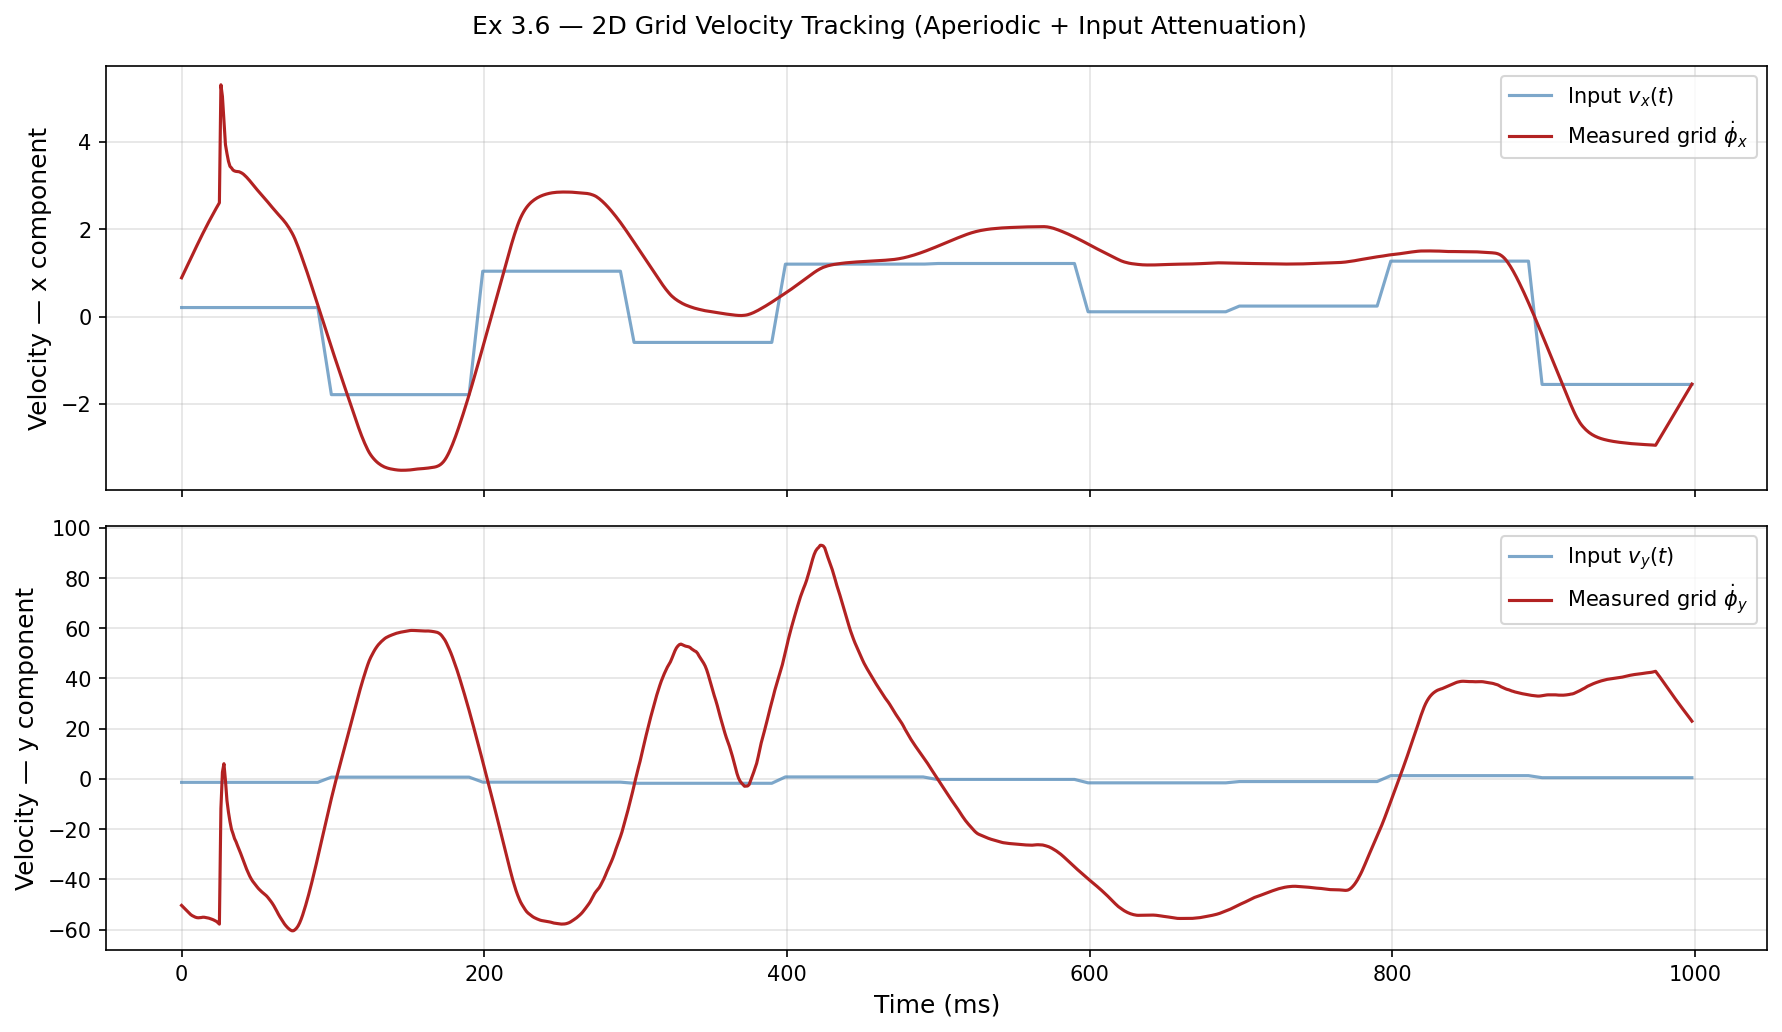
\includegraphics[width=\textwidth]{images2/fig_3_6_velocity_tracking.png}
        \caption{Input vs.\ measured grid velocity under aperiodic boundaries with input attenuation. Tracking is qualitatively preserved but exhibits slightly larger transient lags and a reduced gain compared to the periodic case (Ex 2.4).}
        \label{fig:vel_tracking_36}
    \end{minipage}\hfill
    \begin{minipage}{0.53\textwidth}
        \centering
        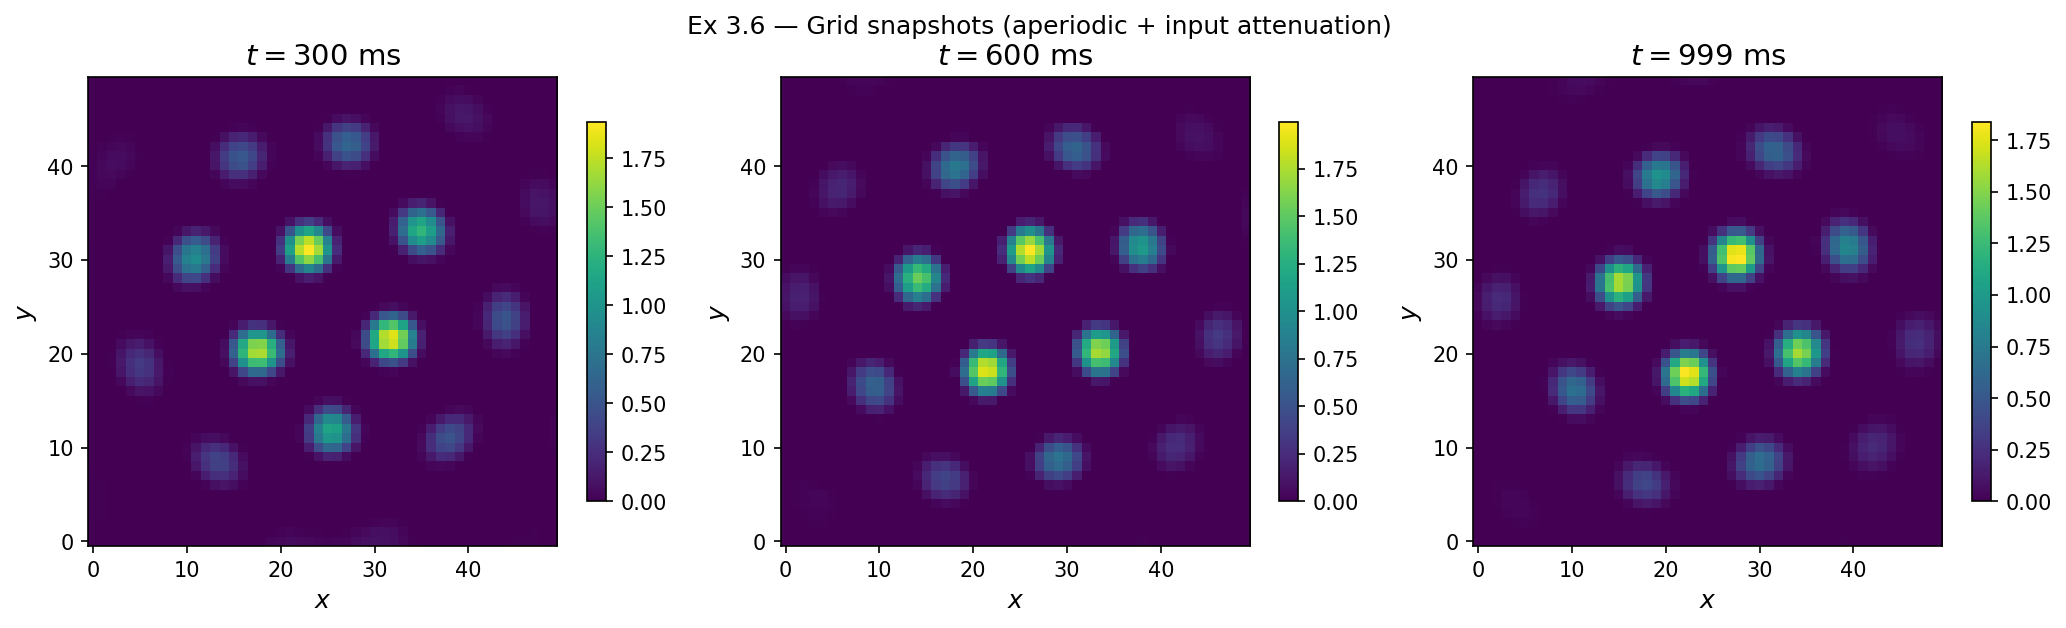
\includegraphics[width=\textwidth]{images2/fig_3_6_snapshots.png}
        \caption{Grid snapshots at $t=300$, 600, 999 ms. The hexagonal lattice is stable in the central region; the peripheral annulus remains quiescent throughout.}
        \label{fig:snapshots_36}
    \end{minipage}
\end{figure}

\textbf{Observation.} Velocity tracking is preserved qualitatively, but two effects emerge relative to Ex 2.4: (i) slightly \textbf{larger transient lags} (the reduced effective network size slows attractor responses); and (ii) mild \textbf{gain compression} (the spatially non-uniform driving force imposed by $e(\mathbf{x})$ reduces the integration gain $\kappa$). The hexagonal lattice remains structurally intact in the network interior throughout, with bumps near the envelope boundary showing slightly lower amplitude. This confirms that input attenuation supports 2D path integration under aperiodic conditions, while making the inherent gain-reduction trade-off explicit.

%=============================================================================
\section{Exercise 4 --- Final Question (Biology-Oriented)}
%=============================================================================

\textbf{Model predictions.} The CAN model predicts: (i) the hexagonal grid emerges spontaneously from center-surround recurrent connectivity; (ii) the grid's spatial phase updates linearly by integrating velocity; and (iii) setting $\alpha=0$ preserves the static lattice but abolishes path integration.

\textbf{Proposed experiment.}

\begin{enumerate}[itemsep=1pt, parsep=0pt, topsep=3pt, partopsep=0pt]
    \item \textit{Preparation.} Chronically implant Neuropixels probes in MEC layer~II of rats on a 1D linear track ($L=2$ m). Identify grid cells by spatial periodicity $\lambda$; simultaneously record head-direction and speed cells (presubiculum) to extract ground-truth $\mathbf{v}(t)$.

    \item \textit{Velocity-gain manipulation.} Use closed-loop VR to decouple optic flow from treadmill speed: $\mathbf{v}_{virtual}=\kappa\mathbf{v}_{physical}$. The CAN predicts grid spacing scales as $1/\kappa$, as the integrator accumulates $\kappa v$ instead of $v$.

    \item \textit{Optogenetic perturbation.} Express ChR2 in medial septum (which paces theta-rhythm velocity signals to MEC). In a stationary animal, injecting a synthetic asymmetric drive should force the attractor to translate, inducing a virtual displacement equal to the time-integral of the injected signal.

    \item \textit{Readout.} Decode the instantaneous spatial phase from MEC population activity (population vector estimator). Compare decoded trajectory $x_{neural}(t)$ to actual position $x_{actual}(t)$; systematic drift $\propto t$ reveals structural heterogeneities (mismatches in $\alpha$, $l$, $\sigma_{exc}$).

    \item \textit{Model extensions.} Bridge theory and data with: (a) a theta-rhythm module ($\sim\!8$ Hz) for realistic velocity-signal gating; and (b) a hippocampal place-cell decoder integrating multiple grid modules for unambiguous position readout.
\end{enumerate}


%=============================================================================
\section{Conclusion}
%=============================================================================

We have successfully implemented and analyzed a hierarchical path-integration model, progressing from a 1D ring attractor to a comprehensive 2D continuous attractor network (CAN) that recapitulates the spontaneous emergence and velocity-driven translation of hexagonal firing fields observed in MEC grid cells. Key findings include:

\begin{itemize}[itemsep=0pt, parsep=0pt, topsep=2pt, partopsep=0pt]
    \item The 1D Mexican-hat connectivity profile drives spontaneous pattern formation.
    \item A dual-population architecture structurally converts a scalar velocity signal into a proportional drift of the activity bump.
    \item Generalizing the architecture to 2D with four directionally shifted populations spontaneously generates a hexagonal lattice, representing the network's minimal-energy state.
    \item Applying a radial envelope $e(\mathbf{x})$ via input attenuation successfully restores the lattice in the network interior and strictly preserves the translation invariance required for undistorted dynamic path integration.
\end{itemize}


%=============================================================================
\section{Approach}
%=============================================================================
The team (Yann and Arthur) divided the simulation work into two parts. One implemented the 1D continuous attractor network for Exercises~0 and~1, while the other implemented the 2D extension and boundary-condition analysis for Exercises~2 and~3. After this first split, we systematically reviewed each other's code, reran all simulations together, and harmonized the notation, parameter choices, and plotting style across the notebook.

We wrote the simulation code in Python, using only the equations from the project statement and standard scientific libraries. For Exercises~0 and~1, we first coded the 1D Mexican-hat kernel, then the Euler integration of the ring attractor, then the two shifted subpopulations used for velocity integration, and finally the velocity readout. In Exercise~1.4, we chose to estimate the bump velocity through the phase of the first spatial Fourier component, because the bump lives on a periodic ring and its position is therefore naturally described as an angle rather than by a simple peak index. For each figure, we proceeded incrementally: first verifying that the kernel shape matched expectations, then checking that the firing-rate heatmaps reproduced the expected bump or periodic structure, and finally validating that the measured bump velocity scaled linearly with the imposed velocity.

For Exercises~2 and~3, we followed the same logic: first generalizing the kernel to 2D, then implementing the four directional populations and testing the emergence of the hexagonal grid, then adding constant and time-varying velocity inputs, and finally comparing periodic versus aperiodic boundaries together with the two correction strategies. Here too, we made explicit methodological choices: in the 2D moving-grid analysis we reused Fourier phase tracking because a rigid translation of the lattice is most naturally captured through the phase of its dominant spatial modes, and in the aperiodic-boundary part we implemented both weight attenuation and input attenuation in order to compare a connectivity-based correction with a drive-based correction. We ultimately retained the interpretation that input attenuation is more appropriate for path-integration dynamics because it preserves the recurrent attractor structure better.

We used a Large Language Model only as a support tool, not to generate the scientific content of the project. In practice, we used it to improve the English of the report, make parts of the code clearer and more readable, and occasionally fix minor syntax or plotting issues. Our prompts were therefore focused on code clarity, variable naming, and academic phrasing, rather than on asking for theoretical derivations or ready-made solutions. The modeling choices, debugging, interpretation of the figures, and final scientific conclusions were all done by the two of us.

\newpage
%=============================================================================
% Bibliography
%=============================================================================
\bibliographystyle{ieeetr}
\bibliography{references}

\end{document}
